\documentclass[12pt]{article}

% ------------------------------------------------------------------
% Core math
\usepackage{amsmath, amssymb, amsthm}
% Diagrams
\usepackage{tikz-cd}
\usepackage{tikz}
\usetikzlibrary{arrows.meta, positioning, calc, fit, backgrounds}
% Graphics
\usepackage{graphicx}
% Tables
\usepackage{longtable}
\usepackage{array}
\usepackage{booktabs}
% Page layout
\usepackage[margin=1in]{geometry}
% GrokRxiv sidebar (uses the modern LaTeX hook system, not the obsolete everypage)
\usepackage{xcolor}
\usepackage{mathtools}
\usepackage{stmaryrd}
\usepackage{enumitem}
% References: hyperref loaded as late as possible; cleveref strictly after it.
\usepackage{hyperref}
\usepackage{cleveref}

\hypersetup{
  colorlinks=true,
  linkcolor=blue!55!black,
  citecolor=green!45!black,
  urlcolor=blue!55!black,
  pdftitle={Foundations: The Representation Stack and the Realization Pipeline},
  pdfauthor={Matthew Long}
}

% ------------------------------------------------------------------
% Theorem environments
\newtheorem{theorem}{Theorem}[section]
\newtheorem{proposition}[theorem]{Proposition}
\newtheorem{lemma}[theorem]{Lemma}
\newtheorem{corollary}[theorem]{Corollary}
\theoremstyle{definition}
\newtheorem{definition}[theorem]{Definition}
\newtheorem{axiom}{Axiom}
\newtheorem{ontaxiom}{Ontology Axiom}
\newtheorem{example}[theorem]{Example}
\newtheorem{conjecture}[theorem]{Conjecture}
\theoremstyle{remark}
\newtheorem{remark}[theorem]{Remark}
% cleveref display names for the custom counters
\crefname{axiom}{Axiom}{Axioms}
\Crefname{axiom}{Axiom}{Axioms}
\crefname{ontaxiom}{Ontology Axiom}{Ontology Axioms}
\Crefname{ontaxiom}{Ontology Axiom}{Ontology Axioms}

% ------------------------------------------------------------------
% Notation macros
\newcommand{\Dom}{\mathsf{Dom}}
\newcommand{\Math}{\mathsf{Math}}
\newcommand{\Phys}{\mathsf{Phys}}
\newcommand{\Info}{\mathsf{Info}}
\newcommand{\Rep}{\mathsf{Rep}}
\newcommand{\Meas}{\mathsf{Meas}}
\newcommand{\Gpd}{\mathsf{Gpd}}
\newcommand{\Cat}{\mathsf{Cat}}
\newcommand{\Set}{\mathsf{Set}}
\newcommand{\Vect}{\mathsf{Vect}}
\newcommand{\Bord}{\mathsf{Bord}}
\newcommand{\Real}{\mathrm{Real}}
\newcommand{\Obs}{\mathrm{Obs}}
\newcommand{\Repphys}{\mathrm{Rep}_{\mathrm{phys}}}
\newcommand{\Aut}{\mathrm{Aut}}
\newcommand{\Stab}{\mathrm{Stab}}
\newcommand{\op}{\mathrm{op}}
\newcommand{\per}{\mathrm{per}}
\newcommand{\id}{\mathrm{id}}
\newcommand{\physrep}[1]{\llbracket #1 \rrbracket_{\mathrm{phys}}}
\newcommand{\Sstat}{\mathsf{S}}
\newcommand{\Hstat}{\mathsf{H}}
\newcommand{\Pstat}{\mathsf{P}}
\newcommand{\stO}{\preceq}

% GrokRxiv DOI sidebar (modern shipout hook; page-1 only)
\definecolor{grokgray}{RGB}{110,110,110}
\AddToHook{shipout/background}{%
  \ifnum\value{page}=1
    \begin{tikzpicture}[remember picture, overlay]
      \node[
        rotate=90,
        anchor=south,
        font=\Large\sffamily\bfseries\color{grokgray},
        inner sep=0pt
      ] at ([xshift=38pt, yshift=0.52\paperheight]current page.south west)
      {GrokRxiv:2026.07.foundations-representation-stack\quad
       [\,math.CT\,]\quad
       04 Jul 2026};
    \end{tikzpicture}
  \fi
}

% ------------------------------------------------------------------
\title{\textbf{Foundations: The Representation Stack\\ and the Realization Pipeline}\\[0.6em]
\large Part~I of \emph{A Math$\to$Physics Representation Library}}

\author{Matthew Long \\
\textit{The YonedaAI Collaboration} \\
\textit{YonedaAI Research Collective} \\
Chicago, IL \\
\texttt{research@yonedaai.com} $\cdot$ \url{https://yonedaai.com}}

\date{4 July 2026}

\begin{document}
\maketitle

\begin{abstract}
We initiate a seven-part modular program that formalizes each mathematical
domain as a \emph{physical-representation module}. This first part supplies the
common substrate on which the remaining six build: a disciplined, domain-indexed
formalism for translating mathematical structure into physical representation.
We introduce the category $\Dom$ of mathematical domains, the fibered assignment
$d \mapsto \Math_d$ of structures in each domain, and a target
category $\Phys$ of physical representation objects (state spaces, observable
algebras, process categories, gauge moduli, quantum code spaces, measurement
outcomes). The central data structure is the \emph{representation entry}
$E = (M,P,\tau,\sigma)$: a mathematical object $M$, a proposed physical
representation $P$, a translation datum $\tau$, and---crucially---an
\emph{epistemic status label} $\sigma \in \{\Sstat,\Hstat,\Pstat\}$
(standard / heuristic / speculative). Entries organize into a
\emph{representation prestack} $\Repphys : \Dom^{\op} \to \Gpd$, which becomes a
\emph{representation stack} exactly when local entries glue up to coherent
gauge equivalence. The engine that turns structure into number is the
\emph{realization pipeline}
$\Obs_\alpha(M) = \Obs\bigl(\Real_\alpha(\Phi(M))\bigr)$, governed by four
axioms: Realization, Equivalence, Locality/descent, and Decomposition. Our
principal contributions are: (T1) functoriality of the realization pipeline;
(T2) a descent criterion characterizing when the representation prestack is a
stack; (T3) a \emph{status calculus} making $\{\Sstat,\Hstat,\Pstat\}$ an ordered
commutative monoid under which epistemic reliability is monotone
non-increasing along chains of translations; and (T4) an obstruction theorem
showing that the coarse (gauge-quotiented) representation library fails descent
precisely when nontrivial automorphisms are present. We provide a runnable
Haskell encoding of the stack and pipeline and an idiomatic Lean sketch of the
core types. The framework is deliberately \emph{modular}, not unified: it fixes
the notation, axioms, and status discipline that Parts~II--VI instantiate for
motives/periods, algebraic geometry, algebraic topology, category theory/HoTT,
and sheaves/stacks/gauge, closing the loop in the synthesis Part.
\end{abstract}

\tableofcontents

% ==================================================================
\section{Introduction}
\label{sec:intro}

\subsection{Motivation}

A recurring experience in mathematical physics is that a physical quantity is
not merely \emph{described by} some piece of mathematics but is literally
\emph{obtained} from it by a structured act of realization. A scattering
amplitude is obtained as a period integral of an algebraic form over a chain; a
partition function is obtained as a trace; a topological quantum field theory
(TQFT) assigns a vector space to a manifold and a linear map to a cobordism; a
logical qubit is obtained by encoding into a larger physical Hilbert space. In
each case a mathematical object $M$ is passed through a pipeline
\[
\begin{aligned}
  M &\xrightarrow{\ \Phi\ } \text{abstract physical information}
     \xrightarrow{\ \Real_\alpha\ } \text{physical representation}\\
    &\xrightarrow{\ \Obs\ } \text{measurement data,}
\end{aligned}
\]
and what we call an ``observable'' is the endpoint of this pipeline. The
guiding slogan of the entire program is compressed as
\[
  \boxed{\ \text{observable} \;=\; \Real(\text{abstract structure}).\ }
\]

This paper does \emph{not} claim that all of physics is a functor out of all of
mathematics. Such a single universal functor is almost certainly not
well-defined. Instead we take the opposite, deliberately modest stance: the
translation is \emph{local} and \emph{domain-indexed}, and every translation
carries an explicit \emph{epistemic status label} recording whether it is a
standard mathematical fact, a strong heuristic, or a speculative ontological
proposal. The status label is part of the formalism, not decoration. It is the
device by which the framework remains honest about what it has actually
established versus what it merely suggests.

\subsection{The modular series}

This is Part~I of a seven-part modular series, \emph{A Math$\to$Physics
Representation Library}. We stress the word \emph{modular}: this is not a
single monolithic theory but a ladder of standalone modules, each readable and
defensible on its own, whose composition is exhibited as an explicit
hierarchical building process rather than asserted as an already-unified whole.
The ladder is summarized in \Cref{tab:ladder}.

\begin{table}[htbp]
\centering
\small
\begin{tabular}{@{}c>{\raggedright\arraybackslash}p{3.4cm}>{\raggedright\arraybackslash}p{7.3cm}@{}}
\toprule
\textbf{Part} & \textbf{Topic} & \textbf{Structure introduced / emergent property} \\
\midrule
I & Foundations (this paper) & $\Dom,\Math_d,\Phys$; representation entries $(M,P,\tau,\sigma)$; prestack/stack; realization pipeline $\Obs\circ\Real_\alpha\circ\Phi$; status system $\Sstat/\Hstat/\Pstat$. \emph{Disciplined translation as data.} \\
II & Motives, periods, amplitudes & Motives $\mathrm{Mot}(X)$, period data $\Pi=(X,D,\omega,\Gamma)$, motivic amplitude objects $\mathcal{A}^{\mathfrak m}$, coproduct $\Delta$, cobracket $\delta$. \emph{$\Real_\alpha$ made concrete and numeric.} \\
III & Algebraic geometry & Schemes, moduli stacks, positive geometries, Hodge structures, Gauss--Manin. \emph{Possibility spaces as geometry.} \\
IV & Algebraic topology & (Co)homology, characteristic classes, bordism, TQFT as $\Bord_n \to \Vect$. \emph{Functorial realization; conserved global data.} \\
V & Category theory \& HoTT & Categories, functors, monoidal/dagger-compact structure, univalence. \emph{The universal grammar; equivalence becomes identity.} \\
VI & Sheaves, stacks, gauge, quantum HA & Stacks as pseudofunctors, gauge redundancy $[X/G]$, quantum high-availability codes, Hopf-algebraic renormalization. \emph{Many representatives, one logical content.} \\
Synth. & Recomposition & Reassembly of I--VI into one conjectural ontology plus limitations. \emph{The ladder closes on Part~I.} \\
\bottomrule
\end{tabular}
\caption{The modular composition ladder. Each part introduces new structure and
adds an emergent property that the composition makes available.}
\label{tab:ladder}
\end{table}

A structural fact worth stating at the outset: the ladder is \emph{circular}.
Part~I \emph{posits} that representation entries behave like a stack---local
data gluing not on the nose but up to equivalence. Part~VI \emph{proves} what a
stack actually is (a fibered category satisfying descent) and shows that
$\Repphys$ is stack-like exactly when compatible local entries glue up to gauge
equivalence. Thus Part~VI supplies the rigorous foundation for Part~I's opening
formalism; the synthesis Part records this as a ``closure theorem.'' We
therefore write Part~I with explicit forward references, flagging every
promissory note that a later module discharges.

\subsection{Contributions}

The concrete contributions of this paper are:

\begin{enumerate}[leftmargin=2.2em]
\item A precise definition of the objects $\Dom$, $\Math_d$, $\Phys$ and the
  bracket notation $\physrep{M}$ for the physical representation of $M$
  (\Cref{sec:framework}).
\item The four core definitions of the representation-stack formalism:
  \emph{representation entry}, \emph{representation library},
  \emph{representation prestack}, and \emph{representation stack}
  (\Cref{sec:stack}), together with the master diagram
  (\Cref{fig:master}).
\item The \emph{realization pipeline} $\Obs_\alpha = \Obs\circ\Real_\alpha\circ\Phi$
  and its four governing axioms (\Cref{sec:pipeline}), plus the parallel
  six-axiom \emph{ontology} presentation and its central conjecture
  (\Cref{sec:ontology}).
\item Four results with proofs: functoriality of the pipeline
  (\Cref{thm:functorial}, a proposition), the descent characterization of
  stackhood (\Cref{thm:descent}), the status calculus (\Cref{thm:status}), and
  the coarse-quotient obstruction (\Cref{thm:coarse}), collected in
  \Cref{sec:results}.
\item The core translation library and two cross-cutting tables
  (operations $\leftrightarrow$ physical interpretation; domains $\leftrightarrow$
  physical faculties) that every later module reuses (\Cref{sec:library}).
\item A runnable Haskell encoding and an idiomatic Lean sketch of the stack and
  pipeline (\Cref{sec:code}).
\end{enumerate}

\subsection{Epistemic status system}
\label{sec:status-intro}

Throughout, every dictionary entry and every proposed correspondence carries
one of three labels, used \emph{verbatim} across all seven parts.

\begin{center}
\begin{tabular}{@{}c>{\raggedright\arraybackslash}p{6.0cm}>{\raggedright\arraybackslash}p{5.6cm}@{}}
\toprule
\textbf{Label} & \textbf{Meaning} & \textbf{Canonical example} \\
\midrule
$\Sstat$ & standard use in mathematics or mathematical physics & TQFT as a functor $\Bord_n \to \Vect$ \\
$\Hstat$ & strong heuristic representation-dictionary entry & motive as ``functional essence'' \\
$\Pstat$ & speculative philosophical ontology & reality as motivic-categorical realization \\
\bottomrule
\end{tabular}
\end{center}

Composite labels ($\Sstat/\Hstat$, $\Hstat/\Pstat$) appear where an entry is
standard as pure mathematics but heuristic or speculative in its physical
reading; we preserve these composites verbatim. \Cref{thm:status} promotes this
informal system to a genuine algebraic calculus.

\subsection{Outline}

\Cref{sec:framework} fixes the categorical framework.
\Cref{sec:stack} defines the representation stack.
\Cref{sec:pipeline} defines the realization pipeline and its axioms.
\Cref{sec:ontology} presents the ontology axioms and the closure conjecture.
\Cref{sec:results} proves the four main theorems.
\Cref{sec:library} reproduces the core translation library.
\Cref{sec:parts} sets up Parts~II--VI as concrete instantiations.
\Cref{sec:code} presents the Haskell and Lean formalizations.
\Cref{sec:discussion} discusses limitations, and \Cref{sec:conclusion}
concludes with the four slogans of the program.

% ==================================================================
\section{Mathematical Framework}
\label{sec:framework}

We work throughout with (possibly higher) categories. For definiteness a reader
may take all categories to be ordinary $1$-categories on first reading and
reinterpret $\Gpd$, $\Cat$ as $(2,1)$- and $2$-categories where the text says
``pseudofunctor'' or ``up to coherent isomorphism.'' Part~V makes the higher
structure precise; here we need only the following ingredients.

\subsection{Domains, structures, and physical targets}

\begin{definition}[Domain category]
\label{def:dom}
The \emph{domain category} $\Dom$ has as objects mathematical domains---%
algebraic topology, algebraic geometry, category theory, homotopy type theory,
sheaf/stack theory, motivic period theory, and so on---and as morphisms
$u : e \to d$ the \emph{refinements}: inclusions of a subdomain, restrictions of
scope, or specialization functors that express ``$e$ is a more local or more
special context inside $d$.'' Composition is composition of refinements and each
domain has an identity refinement.
\end{definition}

\begin{definition}[Structures in a domain]
\label{def:mathd}
For each $d \in \Dom$ let $\Math_d$ be a category (or higher category) whose
objects are the mathematical structures native to $d$ and whose morphisms are
the structure-preserving maps of $d$. A refinement $u : e \to d$ induces a
\emph{restriction functor} $u^\ast : \Math_d \to \Math_e$ (read: view a
$d$-structure through the more special context $e$). We do not require the
$\Math_d$ to be glued into a single category; the whole point of modularity is
that they are indexed by $\Dom$ and related only by the refinement functors.
\end{definition}

\begin{definition}[Physical target category]
\label{def:phys}
$\Phys$ is a category (in general a bicategory or $\infty$-category) of
\emph{physical representation targets}. Representative objects include:
state spaces (Hilbert spaces, phase spaces), observable algebras
($C^\ast$- or von Neumann algebras), process categories (categories of
histories or channels), gauge moduli (quotient stacks of field configurations),
quantum code spaces (logical subsystems of a physical Hilbert space), and
measurement-outcome sets. Morphisms are the physically meaningful maps between
such targets: isometries, $\ast$-homomorphisms, completely positive maps,
gauge-equivariant maps, and so on.
\end{definition}

\begin{definition}[Physical-representation bracket]
\label{def:bracket}
Given a chosen interpretation, we write
\[
  \physrep{M} \in \Phys
\]
for the physical representation assigned to a mathematical structure
$M \in \Math_d$. The bracket is a partial, interpretation-dependent operation:
$\physrep{M}$ is defined only when an entry supplying it has been declared, and
its epistemic reliability is exactly the status of that entry.
\end{definition}

\subsection{Realization channels}

The passage from abstract information to a concrete physical representation is
not unique: the same abstract object can be realized through different
\emph{channels}. We index channels by a symbol $\alpha$.

\begin{definition}[Realization channel]
\label{def:channel}
A \emph{realization channel} is an index $\alpha$ drawn from
\[
\begin{aligned}
  \mathsf{Chan} = \{\,&\text{Betti},\ \text{de Rham},\ \text{Hodge},\ \text{\'etale},\ p\text{-adic},\ \text{quantum},\\
  &\text{thermodynamic},\ \text{computational},\ \text{experimental},\ \text{operational}\,\},
\end{aligned}
\]
together with a functor $\Real_\alpha : \Info_d \to \Rep_d$ from a category of
abstract-information objects to a category of physical representations. Different
$\alpha$ realize the same abstract object into different but comparable physical
data; comparison morphisms between channels are the \emph{comparison isomorphisms}
(e.g.\ the period pairing relating Betti and de Rham channels in Part~II).
\end{definition}

\subsection{The groupoid-valued assignment}

\begin{definition}[Groupoid of entries]
\label{def:gpd-entries}
For $d \in \Dom$, let $\Repphys(d)$ be the \emph{groupoid} whose objects are the
representation entries native to $d$ (\Cref{def:entry} below) and whose morphisms
are the \emph{equivalences} of entries---isomorphisms of the underlying
mathematical structures that are compatible with the translation data and that
represent physically irrelevant changes (dualities, gauge changes, code
stabilizers, changes of coordinates). We take a groupoid rather than a category
because, at the level of representation \emph{content}, only invertible identifications
are physically meaningful; non-invertible processes live in $\Phys$, not among
the entries.
\end{definition}

The assignment $d \mapsto \Repphys(d)$, together with the restriction functors
induced by refinements, is the pseudofunctor
$\Repphys : \Dom^{\op} \to \Gpd$ that we make precise in \Cref{sec:stack}. The
final ingredient we shall need is a notion of covering.

\begin{definition}[Coverage on $\Dom$]
\label{def:coverage}
A \emph{Grothendieck topology} (or coverage) $J$ on $\Dom$ assigns to each domain
$d$ a collection of \emph{covering families} $\{u_i : e_i \to d\}_{i \in I}$ of
refinements, closed under composition, base change, and containing all
isomorphisms, and interpreted physically as: ``the local contexts $e_i$ jointly
exhaust the content of $d$.'' We call the pair $(\Dom, J)$ a \emph{site of
domains}. Coverage encodes ``contextual coverage'': a family of special or local
mathematical viewpoints that together determine the global one.
\end{definition}

% ==================================================================
\section{The Representation Stack}
\label{sec:stack}

We now give the four definitions at the heart of the formalism. They are stated
so as to be independent of the higher-categorical subtleties; \Cref{sec:results}
supplies the theorems that make them useful, and Part~VI supplies the full
descent-theoretic underpinning.

\begin{definition}[Representation entry]
\label{def:entry}
A \emph{representation entry} is a quadruple
\[
  E = (M, P, \tau, \sigma),
\]
where $M \in \Math_d$ is a mathematical structure, $P \in \Phys$ is a proposed
physical representation, $\tau$ is a \emph{semantic translation datum}, and
$\sigma \in \{\Sstat, \Hstat, \Pstat\}$ is the epistemic status label. The
translation datum $\tau$ may be a functor $\Math_d \to \Phys$, a natural
transformation between such, an equivalence class of models, a physical
interpretation map, or a weaker relation; the strength of $\tau$ is exactly what
$\sigma$ records.
\end{definition}

We formalize the graded strength of $\tau$ explicitly, because it is what the
status calculus (\Cref{thm:status}) tracks.

\begin{definition}[Translation strength]
\label{def:transl}
A translation datum $\tau$ from $M \in \Math_d$ to $P \in \Phys$ is one of the
following, listed in decreasing strength:
\begin{enumerate}[leftmargin=2.4em]
\item a \emph{functorial translation}: an actual functor $F : \Math_d \to \Phys$
  with $F(M) \cong P$ (candidate status $\Sstat$);
\item a \emph{natural translation}: a natural transformation between declared
  functors witnessing $M \rightsquigarrow P$ (candidate status $\Sstat/\Hstat$);
\item an \emph{interpretive rule}: a partial assignment $M \mapsto P$ justified
  by analogy or dictionary (candidate status $\Hstat$);
\item a \emph{speculative map}: a proposed but unconstructed assignment
  (candidate status $\Pstat$).
\end{enumerate}
The word ``candidate'' is deliberate: the actual label $\sigma$ of an entry is
assigned by the author and may be weaker than the nominal strength of $\tau$
(e.g.\ a genuine functor whose \emph{physical interpretation} is only heuristic
carries a composite label $\Sstat/\Hstat$).
\end{definition}

\begin{definition}[Representation library]
\label{def:library}
A \emph{mathematics-to-physics representation library} is a collection
$\mathcal{L}$ of representation entries that is closed, whenever the operations
are defined, under:
\begin{enumerate}[leftmargin=2.4em]
\item \emph{restriction} to subdomains along refinements $u : e \to d$;
\item \emph{transport} along equivalences of mathematical structures;
\item \emph{composition} of compatible translations;
\item \emph{decomposition} through boundary, coproduct, or localization
  operations;
\item \emph{realization} into observables via the pipeline of
  \Cref{sec:pipeline}.
\end{enumerate}
\end{definition}

\begin{definition}[Representation prestack]
\label{def:prestack}
A \emph{representation prestack} is a pseudofunctor
\[
  \Repphys : \Dom^{\op} \longrightarrow \Gpd
\]
assigning to each domain $d$ the groupoid $\Repphys(d)$ of representation entries
(\Cref{def:gpd-entries}) and to each refinement $u : e \to d$ a restriction
functor $u^\ast : \Repphys(d) \to \Repphys(e)$, together with coherent
composition isomorphisms $\gamma_{u,v} : (u v)^\ast \Rightarrow v^\ast u^\ast$
satisfying the pseudofunctor cocycle conditions.
\end{definition}

\begin{definition}[Representation stack]
\label{def:stack}
Let $(\Dom, J)$ be a site of domains. A representation prestack $\Repphys$ is a
\emph{representation stack} if, for every covering family
$\{u_i : e_i \to d\}_{i \in I} \in J(d)$, compatible families of local
representation entries glue to a global entry uniquely up to coherent
isomorphism; equivalently (\Cref{thm:descent}), the comparison functor from
$\Repphys(d)$ to the groupoid of $J$-descent data is an equivalence.
\end{definition}

\begin{remark}
\label{rem:stack-broad}
The word ``stack'' is used broadly. The groupoids $\Repphys(d)$ record
physically irrelevant equivalences: gauge changes, duality transformations,
code stabilizers, or changes of coordinates. Part~I
\emph{posits} this stack-like behavior by analogy; Part~VI supplies its rigorous
descent-theoretic meaning. The reader should treat \Cref{def:stack} as a
promissory note whose payment is scheduled for Part~VI, and \Cref{thm:descent}
as the interface contract between them.
\end{remark}

\subsection{The master diagram}

The canonical picture of the entire program is the following five-node pipeline,
with a feedback loop expressing that gauge/equivalence/duality-related structures
enter the pipeline as the \emph{same} abstract information.

\begin{figure}[htbp]
\centering
\resizebox{\textwidth}{!}{%
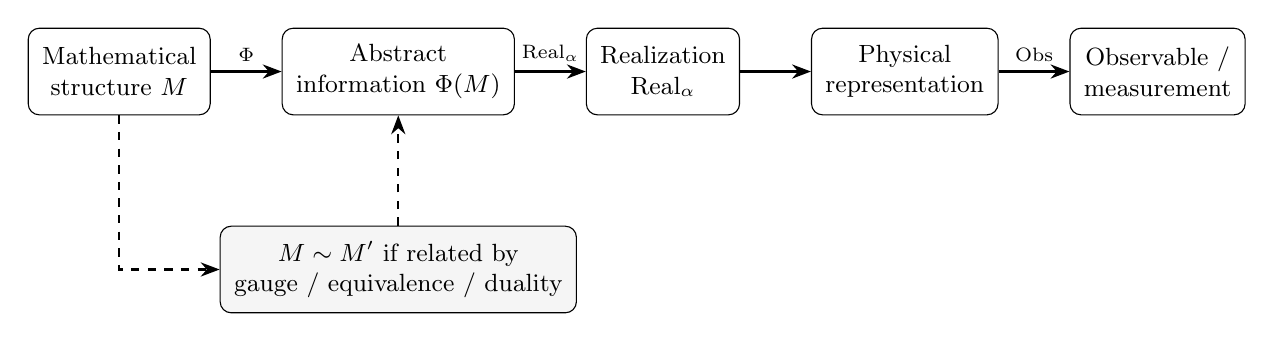
\begin{tikzpicture}[
  node distance=6mm and 9mm,
  box/.style={draw, rounded corners, align=center, minimum height=11mm,
              inner xsep=5pt, font=\small},
  every edge/.style={draw, -{Stealth[length=2.4mm]}, thick},
]
\node[box] (M)   {Mathematical\\ structure $M$};
\node[box, right=of M]   (Phi) {Abstract\\ information $\Phi(M)$};
\node[box, right=of Phi] (Rl)  {Realization\\ $\Real_\alpha$};
\node[box, right=of Rl]  (Prep){Physical\\ representation};
\node[box, right=of Prep](Ob)  {Observable /\\ measurement};

\path (M)   edge node[above,font=\scriptsize] {$\Phi$}   (Phi);
\path (Phi) edge node[above,font=\scriptsize] {$\Real_\alpha$} (Rl);
\path (Rl)  edge (Prep);
\path (Prep) edge node[above,font=\scriptsize] {$\Obs$} (Ob);

\node[box, below=14mm of Phi, fill=gray!8] (equiv)
  {$M \sim M'$ if related by\\ gauge / equivalence / duality};
\draw[-{Stealth[length=2.4mm]}, thick, dashed] (equiv) -- (Phi);
\draw[-{Stealth[length=2.4mm]}, thick, dashed] (M.south) |- (equiv.west);
\end{tikzpicture}%
}
\caption{The master diagram of the realization pipeline. A mathematical
structure $M$ is sent by $\Phi$ to abstract physical information, realized
through a channel $\Real_\alpha$ into a physical representation, from which
$\Obs$ extracts measurement data. The dashed feedback expresses the Equivalence
axiom: structures related by gauge, equivalence, or duality feed identical
abstract information into the pipeline.}
\label{fig:master}
\end{figure}

The same pipeline can be drawn as a commuting diagram of categories, which is the
form used in \Cref{thm:functorial}:
\[
\begin{tikzcd}[column sep=large]
\Math_d \arrow[r, "\Phi"] \arrow[rrr, bend right=22, "\Obs_\alpha"'] &
\Info_d \arrow[r, "\Real_\alpha"] &
\Rep_d \arrow[r, "\Obs"] &
\Meas_d
\end{tikzcd}
\]

% ==================================================================
\section{The Realization Pipeline}
\label{sec:pipeline}

\begin{definition}[Realization pipeline]
\label{def:pipeline}
Fix a domain $d$ and a channel $\alpha$. The \emph{realization pipeline} is the
composite
\[
  \Obs_\alpha \;=\; \Obs \circ \Real_\alpha \circ \Phi \;:\;
  \Math_d \xrightarrow{\ \Phi\ } \Info_d \xrightarrow{\ \Real_\alpha\ }
  \Rep_d \xrightarrow{\ \Obs\ } \Meas_d,
\]
where $\Phi$ extracts the abstract physical-information content of a structure,
$\Real_\alpha$ realizes it into a physical representation through channel
$\alpha$, and $\Obs$ extracts measurement data. On objects,
\[
  \Obs_\alpha(M) \;=\; \Obs\bigl(\Real_\alpha(\Phi(M))\bigr).
\]
\end{definition}

The pipeline is governed by four axioms. These are the axioms every later module
instantiates concretely.

\begin{axiom}[Realization]
\label{ax:real}
Every observable is the output of the pipeline:
$\text{observable} = \Obs \circ \Real_\alpha(\text{abstract structure})$. There
is no observable content except through a declared channel $\alpha$.
\end{axiom}

\begin{axiom}[Equivalence]
\label{ax:equiv}
Mathematical descriptions related by an equivalence lying in the
automorphism/gauge groupoid of a representation entry determine the \emph{same}
physical content at the chosen observational level. Formally, if
$g : M \xrightarrow{\sim} M'$ is a morphism in the groupoid $\Repphys(d)$ then
there is a canonical isomorphism $\Obs_\alpha(M) \cong \Obs_\alpha(M')$ in
$\Meas_d$; when $\Meas_d$ is skeletal (e.g.\ a bare set of numerical measurement
outcomes) this canonical isomorphism is a genuine equality
$\Obs_\alpha(M) = \Obs_\alpha(M')$.
\end{axiom}

\begin{axiom}[Locality / descent]
\label{ax:local}
Physical representations must be locally assignable and globally coherent: for a
covering $\{e_i \to d\}$, a global representation is determined by compatible
local ones. Failure of descent is not a defect of the formalism but a physical
phenomenon---an obstruction, anomaly, or missing boundary datum.
\end{axiom}

\begin{axiom}[Decomposition]
\label{ax:decomp}
Compositional or period-like observables admit a decomposition operation
(boundary $\partial$, coproduct $\Delta$, coaction, spectral sequence, or
factorization) revealing lower-level informational pieces. The decomposition is
functorial: it commutes with compatible realization channels.
\end{axiom}

\begin{example}[TQFT as a status-$\Sstat$ pipeline]
\label{ex:tqft}
Let $d$ be algebraic topology and take $\Phi$ to send an $n$-manifold to its
bordism data, $\Real_\alpha$ to be a fixed TQFT functor
$Z : \Bord_n \to \Vect$, and $\Obs$ to read off partition functions and
correlation numbers. Then $\Obs_\alpha$ is an honest functor and the entry
carries status $\Sstat$: the realization is an actually-constructed functor.
This is the paradigm the other modules aim to emulate. It is developed fully in
Part~IV.
\end{example}

\begin{example}[A status-$\Hstat$ pipeline]
\label{ex:motive}
Let $d$ be motivic period theory, $\Phi$ send a variety $X$ to its motive
$\mathrm{Mot}(X)$ read as ``functional essence,'' $\Real_\alpha$ be a period
realization, and $\Obs$ take numerical periods. The mathematics of realization
functors on motives is standard (status $\Sstat$ \emph{as mathematics}), but the
reading of the motive as the physical ``functional essence'' of $X$ is
heuristic, so the \emph{entry} carries the composite label $\Sstat/\Hstat$. This
is developed in Part~II, where the caution that a motive is not literally ``the
functions of'' $X$ is stated prominently.
\end{example}

% ==================================================================
\section{Axioms for a Representation Ontology}
\label{sec:ontology}

The four pipeline axioms of \Cref{sec:pipeline} are operational. The source
program also presents a parallel, more philosophical set of six \emph{ontology}
axioms, which we reproduce because the synthesis Part treats them as the target
statement the whole ladder discharges. We then note their relationship to the
pipeline axioms.

\begin{ontaxiom}[Syntax]
\label{ax:syntax}
Mathematics is the syntax of physical representation: physical systems, states,
and processes are carried by mathematical structures $M \in \Math_d$.
\end{ontaxiom}

\begin{ontaxiom}[Semantics]
\label{ax:semantics}
The functional essence of a structure---its invariant pre-numerical content---is
its semantics; in Part~II this is made precise as a motive.
\end{ontaxiom}

\begin{ontaxiom}[Realization (ontological)]
\label{ax:real-ont}
Observables arise by realizing semantic content through a channel:
$\Obs_\alpha(M) = \Obs(\Real_\alpha(\Phi(M)))$. This is \Cref{ax:real} read
ontologically.
\end{ontaxiom}

\begin{ontaxiom}[Equivalence / gauge]
\label{ax:equiv-ont}
Descriptions differing by gauge, equivalence, or duality determine the same
physical content; this is \Cref{ax:equiv} read ontologically and is discharged
type-theoretically (univalence, Part~V) and geometrically (descent, Part~VI).
\end{ontaxiom}

\begin{ontaxiom}[Decomposition (ontological)]
\label{ax:decomp-ont}
Observable content decomposes into primitive informational pieces via a
coalgebraic operation; this is \Cref{ax:decomp} read ontologically and is made
concrete by the Goncharov coproduct (Part~II) and Connes--Kreimer coproduct
(Part~VI).
\end{ontaxiom}

\begin{ontaxiom}[Motivic pre-numericality]
\label{ax:motivic}
Numbers extracted from physics are realizations of pre-numerical motivic data:
$\mathcal{A} = \per(\mathcal{A}^{\mathfrak m})$. This is the amplitude-level
refinement of \Cref{ax:real}; it drives Part~II.
\end{ontaxiom}

\begin{conjecture}[Motivic-categorical information ontology]
\label{conj:closure}
A sufficiently broad class of physical theories admits a representation-stack
description in which states, processes, observables, amplitudes, gauge
redundancies, and measurement values arise as realizations of structured
categorical, homotopical, geometric, and motivic information. Equivalently, for
such theories the prestack $\Repphys$ built from the modules of Parts~II--VI is a
representation stack in the sense of \Cref{def:stack}.
\end{conjecture}

\begin{remark}[Relationship of the two axiom sets]
The pipeline axioms (\Cref{ax:real}--\Cref{ax:decomp}) are what one \emph{uses}
to build entries; the ontology axioms (\Cref{ax:syntax}--\Cref{ax:motivic}) are
what one \emph{claims} the entries collectively mean. \Cref{ax:real} and
\Cref{ax:real-ont} coincide; \Cref{ax:equiv} and \Cref{ax:equiv-ont} coincide;
\Cref{ax:decomp} and \Cref{ax:decomp-ont} coincide; the Locality axiom
(\Cref{ax:local}) is the operational shadow of \Cref{conj:closure}'s demand that
$\Repphys$ be a \emph{stack}, i.e.\ that descent hold. \Cref{ax:syntax},
\Cref{ax:semantics}, and \Cref{ax:motivic} have no operational counterpart in
\Cref{sec:pipeline}; they are the semantic layer Part~II supplies.
\end{remark}

% ==================================================================
\section{Results}
\label{sec:results}

We prove the four main results. \Cref{thm:functorial} and \Cref{thm:descent}
concern the pipeline and the stack; \Cref{thm:status} turns the status system
into a calculus; \Cref{thm:coarse} is the first appearance of the ``stacks
retain gauge information'' phenomenon that recurs across the whole series.

\subsection{Functoriality of the realization pipeline}

\begin{proposition}[Functoriality of the realization pipeline]
\label{thm:functorial}
Fix a domain $d$ and a channel $\alpha$. Suppose the three stages
\[
  \Phi : \Math_d \to \Info_d, \qquad
  \Real_\alpha : \Info_d \to \Rep_d, \qquad
  \Obs : \Rep_d \to \Meas_d
\]
are each functors. Then the assignment
$M \mapsto \Obs_\alpha(M) = \Obs(\Real_\alpha(\Phi(M)))$ extends to a functor
$\Obs_\alpha : \Math_d \to \Meas_d$. Moreover the assignment
$\alpha \mapsto \Obs_\alpha$ is functorial in the channel: a comparison
morphism $\theta : \alpha \Rightarrow \beta$ (a natural transformation
$\Real_\alpha \Rightarrow \Real_\beta$) induces a natural transformation
$\Obs_\alpha \Rightarrow \Obs_\beta$.
\end{proposition}

\begin{proof}
The composite of functors is a functor: on objects,
$(\Obs \circ \Real_\alpha \circ \Phi)(M)$ is defined as above; on a morphism
$f : M \to M'$ set
$\Obs_\alpha(f) = \Obs(\Real_\alpha(\Phi(f)))$. Functoriality is inherited
stagewise. Identities:
$\Obs_\alpha(\id_M) = \Obs(\Real_\alpha(\Phi(\id_M))) =
\Obs(\Real_\alpha(\id_{\Phi M})) = \Obs(\id_{\Real_\alpha\Phi M}) =
\id_{\Obs_\alpha M}$, using that each stage preserves identities. Composition:
for $f : M \to M'$, $g : M' \to M''$,
\[
\begin{aligned}
  \Obs_\alpha(g \circ f)
  &= \Obs\Real_\alpha\Phi(g \circ f)
   = \Obs\Real_\alpha\bigl(\Phi(g)\circ\Phi(f)\bigr)\\
  &= \Obs\bigl(\Real_\alpha\Phi(g) \circ \Real_\alpha\Phi(f)\bigr)
   = \Obs_\alpha(g)\circ\Obs_\alpha(f),
\end{aligned}
\]
again stagewise. Hence $\Obs_\alpha$ is a functor. For the second claim, let
$\theta : \Real_\alpha \Rightarrow \Real_\beta$ be natural. Define
$\Theta_M := \Obs(\theta_{\Phi M}) : \Obs_\alpha(M) \to \Obs_\beta(M)$. For
$f : M \to M'$ naturality of $\theta$ at $\Phi(f)$ gives
$\theta_{\Phi M'} \circ \Real_\alpha\Phi(f) = \Real_\beta\Phi(f) \circ
\theta_{\Phi M}$; applying the functor $\Obs$ and using its functoriality yields
$\Theta_{M'} \circ \Obs_\alpha(f) = \Obs_\beta(f) \circ \Theta_M$, i.e.\ $\Theta$
is natural. Concretely $\Theta = \Obs \ast \theta \ast \Phi$ is the horizontal
composition (whiskering / Godement product) of $\theta$ with the functors $\Obs$
and $\Phi$, so its naturality is the standard $2$-categorical fact that
whiskering a natural transformation by functors yields a natural transformation.
This is exactly the naturality that Part~II's period comparison
(Betti vs.\ de Rham) instantiates.
\end{proof}

\begin{remark}[Where the status labels bite]
\label{rem:status-bite}
\Cref{thm:functorial} is a triviality about functor composition; its \emph{force}
is entirely in the hypothesis that each stage is a functor. An entry earns status
$\Sstat$ precisely when this hypothesis is discharged by an actual construction
(as in \Cref{ex:tqft}). An $\Hstat$- or $\Pstat$-entry only posits the stages,
so the same formula holds \emph{formally} but is not backed by a construction.
The theorem thus makes explicit that ``$\Obs_\alpha$ is a functor'' is a claim
whose reliability equals the status of its weakest stage---which is precisely
what \Cref{thm:status} quantifies.
\end{remark}

\subsection{When is the prestack a stack?}

\begin{theorem}[Descent characterization of stackhood]
\label{thm:descent}
Let $(\Dom, J)$ be a site of domains and $\Repphys : \Dom^{\op} \to \Gpd$ a
representation prestack. Then $\Repphys$ is a representation stack
(\Cref{def:stack}) if and only if for every $d \in \Dom$ and every covering
family $\{u_i : e_i \to d\}_{i \in I} \in J(d)$ the natural comparison functor
\[
  \Lambda_d : \Repphys(d) \longrightarrow \mathrm{Desc}\bigl(J; \{u_i\}; \Repphys\bigr)
\]
into the groupoid of $J$-descent data is an equivalence of groupoids. Here a
descent datum is a family $(E_i)_{i}$ with $E_i \in \Repphys(e_i)$ together with
gluing isomorphisms $\phi_{ij} : \mathrm{pr}_i^\ast E_i \xrightarrow{\sim}
\mathrm{pr}_j^\ast E_j$ on the pairwise overlaps satisfying the cocycle condition
$\phi_{jk}\circ\phi_{ij} = \phi_{ik}$ on triple overlaps (suppressing, as is
standard, the pullbacks of each $\phi$ to the common triple fiber product
$e_i \times_d e_j \times_d e_k$ along the evident projections). Here
$\mathrm{pr}_i : e_i \times_d e_j \to e_i$ and
$\mathrm{pr}_j : e_i \times_d e_j \to e_j$ are the two projections out of the
fiber product (intersection) $e_i \times_d e_j$, which exists by the base-change
closure of the coverage (\Cref{def:coverage}); we use projection subscripts
(not transition-map subscripts) throughout, so $\phi_{ij}$ merely indexes the
ordered overlap $(i,j)$. The triple overlaps are the fiber products
$e_i \times_d e_j \times_d e_k$.
\end{theorem}

\begin{proof}
$(\Rightarrow)$ Suppose $\Repphys$ is a stack. By \Cref{def:stack}, compatible
families of local entries glue to a global entry uniquely up to coherent
isomorphism. ``Compatible family'' is exactly a descent datum; ``glues to a
global entry'' says $\Lambda_d$ is essentially surjective; ``uniquely up to
coherent isomorphism'' says $\Lambda_d$ is fully faithful. Hence $\Lambda_d$ is
an equivalence.

$(\Leftarrow)$ Suppose each $\Lambda_d$ is an equivalence. Essential
surjectivity gives existence of a gluing (every descent datum comes from a global
entry); fullness and faithfulness give uniqueness up to unique compatible
isomorphism. This is \Cref{def:stack}.

We record that the equivalence, when it fails, fails by a controlled amount: the
prestack always admits a \emph{stackification} $\Repphys \to \Repphys^{+}$, the
universal map to a stack, obtained by the plus-construction that formally adjoins
gluings of descent data. $\Repphys$ is already a stack iff the unit
$\Repphys \to \Repphys^{+}$ is an equivalence, iff each $\Lambda_d$ is an
equivalence. The construction of $\Repphys^{+}$ and the verification that it is a
stack are exactly the descent-theoretic content discharged rigorously in Part~VI;
here we use only its universal property, which is what makes the ``if and only
if'' meaningful without circularity.
\end{proof}

\begin{remark}[Forward reference to Part~VI]
\Cref{thm:descent} is stated as an interface. Its right-hand side---the groupoid
$\mathrm{Desc}(J;\{u_i\};\Repphys)$ and the stackification $\Repphys^+$---is
constructed in full in Part~VI, where descent for a Grothendieck topology is
developed properly (following Giraud and Vistoli). Part~I is entitled to
\emph{state} the criterion and to reason with it, because both directions are
formal once ``descent datum'' and ``stackification'' are granted their standard
meanings. This is the precise sense in which Part~VI ``pays'' Part~I's
promissory note.
\end{remark}

\subsection{The status calculus}

We now promote the informal $\Sstat/\Hstat/\Pstat$ system to an algebraic
structure, so that the status of a \emph{composite} translation is computed, not
guessed. Order the labels by reliability,
\[
  \Sstat \stO \Hstat \stO \Pstat,
\]
read ``$\Sstat$ is at least as reliable as $\Hstat$, which is at least as
reliable as $\Pstat$.''

\begin{theorem}[Status calculus]
\label{thm:status}
Let $\Sigma = \{\Sstat, \Hstat, \Pstat\}$ with the total order
$\Sstat \stO \Hstat \stO \Pstat$.
\begin{enumerate}[leftmargin=2.2em]
\item $(\Sigma, \vee, \Sstat)$ is a commutative idempotent monoid, where
  $a \vee b := \max_{\stO}(a,b)$ is the \emph{less reliable} of the two labels
  --- their \emph{join} (supremum) in the reliability order --- and $\Sstat$,
  the $\stO$-least (most reliable) element, is the unit.
\item If representation entries $E_1 = (M_1,P_1,\tau_1,\sigma_1)$ and
  $E_2 = (M_2,P_2,\tau_2,\sigma_2)$ compose (i.e.\ $\tau_2 \circ \tau_1$ is
  defined, so $P_1 = M_2$ in the evident sense), then the composite entry
  $E_2 \circ E_1$ has status
  \[
    \sigma(E_2 \circ E_1) \;=\; \sigma_1 \vee \sigma_2.
  \]
  In particular the status \emph{value} is \emph{monotone non-decreasing} under
  composition in the $\stO$ order---equivalently, \emph{reliability} is monotone
  non-increasing: $\sigma(E_2\circ E_1) \stO \sigma_i$ fails in general, while
  $\sigma_i \stO \sigma(E_2\circ E_1)$ always holds---a chain of translations is
  only as reliable as its weakest link.
\item Regard a representation library $\mathcal{L}$ as a category whose objects
  are \emph{all} the carriers appearing in its entries---the union
  $\Math_d \cup \Info_d \cup \Rep_d \cup \Phys \cup \Meas_d$ of mathematical,
  informational, and physical targets---and whose morphisms are entries under
  composition (so a pipeline stage $\Math_d \to \Info_d$ and an entry
  $\Info_d \to \Rep_d$ compose as morphisms with matching object types), and let
  $B(\Sigma,\vee)$ be the one-object category obtained by delooping the
  status monoid (its unique hom-monoid is $(\Sigma,\vee)$). Then the assignment
  $\sigma : \mathcal{L} \to B(\Sigma,\vee)$ sending each entry to its status
  label is a \emph{functor}; it is the universal composition-respecting,
  $\Sstat$-normalized status invariant.
\end{enumerate}
\end{theorem}

\begin{proof}
(1) $\vee = \max_{\stO}$ on a totally ordered set is associative, commutative,
and idempotent, and the $\stO$-least element $\Sstat$ is its identity:
$\Sstat \vee a = \max_{\stO}(\Sstat, a) = a$. Hence $(\Sigma,\vee,\Sstat)$ is
a commutative idempotent monoid (a bounded join-semilattice with bottom $\Sstat$
and top $\Pstat$).

(2) By the intended semantics of the labels (\Cref{sec:status-intro}): $\Sstat$
asserts that an actual functorial/natural construction exists; $\Hstat$ asserts a
heuristic interpretive rule; $\Pstat$ asserts a speculative claim. A composite
$\tau_2\circ\tau_1$ inherits the constructions of \emph{both} factors, so it can
be no more reliable than the less reliable factor: if either $\tau_i$ is merely
speculative, the composite passes through a speculative step and is speculative;
if the weaker of the two is heuristic and the other standard, the composite is
heuristic; only if both are standard is the composite standard. This is exactly
$\sigma_1 \vee \sigma_2 = \max_{\stO}(\sigma_1,\sigma_2)$. Monotonicity is then
$\sigma_i \stO \max_{\stO}(\sigma_1,\sigma_2)$, which holds by definition of
$\max$.

(3) Composition of entries is associative with units the identity entries
$(M,M,\id,\Sstat)$, so $\mathcal{L}$ is a category. Delooping the commutative
monoid $(\Sigma,\vee,\Sstat)$ yields the one-object category $B(\Sigma,\vee)$
whose single hom-set is $\Sigma$ with composition $\vee$ and identity
$\Sstat$. The assignment $\sigma$ sends every object of $\mathcal{L}$ to the
unique object of $B(\Sigma,\vee)$ and every entry to its label; it preserves
identities, $\sigma(\id) = \Sstat$, and composition,
$\sigma(E_2\circ E_1) = \sigma(E_2)\vee\sigma(E_1)$ by~(2). Hence $\sigma$ is a
functor $\mathcal{L} \to B(\Sigma,\vee)$. (We emphasize that $\mathcal{L}$ is a
genuine category, not a monoid, so the target is the \emph{delooping}
$B(\Sigma,\vee)$ and no monoidal structure on $\mathcal{L}$ is assumed or
needed.) Universality: any composition-respecting, identity-normalized invariant
valued in a totally ordered monoid factors through $\sigma$, because $\sigma$ is
determined on generators (single entries) and extended by $\vee$, which is
forced by~(2).
\end{proof}

\begin{corollary}[Reliability of a pipeline]
\label{cor:pipeline-status}
The status of a realization pipeline $\Obs_\alpha = \Obs\circ\Real_\alpha\circ\Phi$
viewed as a composite of three entries is
$\sigma(\Phi)\vee\sigma(\Real_\alpha)\vee\sigma(\Obs)$. Consequently an
$\Sstat$-labeled pipeline requires \emph{all three} stages to be $\Sstat$; a
single heuristic stage downgrades the whole pipeline to $\Hstat$.
\end{corollary}

\begin{proof}
Immediate from \Cref{thm:status}(2) applied twice and associativity of $\vee$.
This is the formal content of \Cref{rem:status-bite}.
\end{proof}

\begin{remark}
\Cref{thm:status} is original to this program: it operationalizes the paper's
status system into a checkable calculus, valuable for automated (Lean-checked)
status propagation. The Haskell and Lean encodings of \Cref{sec:code} implement
$\vee$ directly, so that composing entries \emph{computes} the composite status
rather than requiring the author to assign it by hand.
\end{remark}

\subsection{Coarse quotients lose gauge information}

The last theorem is the Part~I shadow of a phenomenon that recurs, at increasing
rigor, throughout the series: quotienting away automorphisms destroys descent.

\begin{theorem}[Coarse-quotient obstruction]
\label{thm:coarse}
Suppose $\Repphys$ is a representation stack and let $\pi(d) :=
\pi_0(\Repphys(d))$ be the set of isomorphism classes of entries (the ``coarse''
representation library, obtained by quotienting each groupoid by its gauge
equivalences). Then $d \mapsto \pi(d)$ is a presheaf of sets, but in general it
\emph{can fail} to be a sheaf. Concretely, suppose some entry
$E \in \Repphys(d)$ has a nontrivial automorphism group $\Aut(E) \neq 1$ and the
site is rich enough to admit a covering $\{e_i \to d\}$ supporting a nontrivial
$\Aut(E)$-torsor (equivalently, a nontrivial \v{C}ech $1$-cocycle class valued in
$\Aut(E)$, so that $\check{H}^1(\{e_i\}; \Aut(E)) \neq 0$). Then there is a
covering on which local classes agree on overlaps yet fail to glue to a unique
global class, so $\pi$ is not a sheaf.
\end{theorem}

\begin{proof}
Presheaf: $\pi_0$ is functorial (a functor of groupoids induces a map on
isomorphism-class sets), and restriction functors $u^\ast$ induce restriction
maps $\pi(d) \to \pi(e)$; the pseudofunctor coherence of $\Repphys$ makes these
strictly functorial after passing to $\pi_0$ (all $2$-cells become identities on
$\pi_0$). Hence $\pi$ is a presheaf.

Failure of the sheaf condition: pick $E \in \Repphys(d)$ with a nontrivial
automorphism $g \in \Aut(E)$, and choose a covering $\{u_i : e_i \to d\}$ that is
``fine enough'' that $g$ becomes locally trivializable, i.e.\ each restriction
$u_i^\ast g$ is isotopic to the identity in $\Repphys(e_i)$ while $g$ itself is
not the identity globally. (Such a covering exists whenever the automorphism is
supported by the gluing data---this is the generic situation for gauge
automorphisms; in Part~VI this is realized concretely for $[X/G]$-type stacks
with $G$ acting with stabilizers.) Let $E^{g}$ be the distinct global entry
obtained by regluing the \emph{same} local data $(u_i^\ast E)_i$ along the
descent datum twisted by the nontrivial $1$-cocycle valued in $\Aut(E)$
determined by $g$ (a ``twisted sector''). Then $E$ and $E^{g}$ have equal
restrictions to every $e_i$ and equal overlap comparisons in $\pi_0$, hence
define the \emph{same} element of the sheaf of local sections of $\pi$; but
$E \not\cong E^{g}$ as global entries, since the nontrivial cocycle
class obstructs a global identification when $g \neq \id$. Thus the section over
$\{e_i\}$ has (at least) two preimages in $\pi(d)$, violating the uniqueness
half of the sheaf axiom. Existence can fail dually. Therefore $\pi$ is not a
sheaf.
\end{proof}

\begin{corollary}
\label{cor:stack-informative}
The stack $\Repphys$ is strictly more informative than its coarse library
$\pi$: passing to $\pi$ forgets exactly the automorphism (gauge/stabilizer) data,
and this data is what descent requires. Retaining it is the entire reason the
formalism is built on groupoid-valued (stack) rather than set-valued (sheaf)
assignments.
\end{corollary}

\begin{proof}
By \Cref{thm:coarse}, $\pi$ fails descent exactly where $\Repphys$ has nontrivial
automorphisms; since $\Repphys$ satisfies descent by hypothesis, the difference
between them is precisely the retained automorphism data. This is the Part~I
statement of the recurring theorem ``stacks retain gauge information,'' proved
algebro-geometrically in Part~III, type-theoretically in Part~V, and
descent-theoretically in Part~VI.
\end{proof}

% ==================================================================
\section{The Core Translation Library}
\label{sec:library}

We reproduce the foundational dictionary that Parts~II--VI extend. Every row
carries a status label per \Cref{sec:status-intro}. The library is presented as
three tables: the core translation grammar (\Cref{tab:core}), the operations
dictionary (\Cref{tab:ops}), and the domains-as-faculties dictionary
(\Cref{tab:faculties}). These are shared across all seven parts; later modules
cite them rather than restating them.

\begin{longtable}{@{}>{\raggedright\arraybackslash}p{3.5cm}>{\raggedright\arraybackslash}p{4.5cm}>{\raggedright\arraybackslash}p{4.8cm}c@{}}
\caption{Core translation library (foundations grammar).}
\label{tab:core}\\
\toprule
\textbf{Mathematics} & \textbf{Physical representation} & \textbf{Semantic interpretation} & \textbf{Status} \\
\midrule
\endfirsthead
\multicolumn{4}{@{}l}{\small\itshape \Cref{tab:core}, continued}\\
\toprule
\textbf{Mathematics} & \textbf{Physical representation} & \textbf{Semantic interpretation} & \textbf{Status} \\
\midrule
\endhead
\midrule
\multicolumn{4}{r@{}}{\small\itshape continued on next page}\\
\endfoot
\bottomrule
\endlastfoot
Object $X$ & Physical system or world-structure & Structured carrier of physical information & $\Hstat$ \\
Representation $\rho:X\to\mathrm{End}(V)$ & Physical realization on states & How structure acts on observables/states & $\Sstat$ \\
Realization functor & Translation into measurable form & Abstract information to readable data & $\Sstat/\Hstat$ \\
Invariant & Conservation law / observable & What is stable under allowed transformations & $\Sstat$ \\
Equivalence & Same physics, different coordinates & Dual descriptions, gauge equivalence & $\Sstat$ \\
Symmetry & Redundancy or physical transformation & Law-preserving structure & $\Sstat$ \\
Duality & Two theories, same content & Equivalence of representation languages & $\Sstat$ \\
Moduli space & Space of distinct configurations & Parameter space of possible structures & $\Sstat$ \\
Quotient & Identification of redundant descriptions & Gauge reduction or physical state space & $\Sstat$ \\
Boundary & Physical interface / asymptotic region & Where factorization/measurement appears & $\Sstat/\Hstat$ \\
Singularity & Threshold / phase transition & Breakdown or special physical regime & $\Sstat/\Hstat$ \\
Decomposition & Factorization, cut, measurement split & Observable broken into primitive pieces & $\Sstat$ \\
Primitive & Irreducible informational unit & Indecomposable in the chosen grammar & $\Hstat$ \\
Functor & Physical theory as translation & States to spaces, processes to histories & $\Sstat$ \\
Natural transformation & Equivalence/deformation of theories & Consistent translation between descriptions & $\Sstat/\Hstat$ \\
Category & Universe of systems and processes & Objects are systems; morphisms are transitions & $\Sstat/\Hstat$ \\
\end{longtable}

\begin{longtable}{@{}>{\raggedright\arraybackslash}p{4.4cm}>{\raggedright\arraybackslash}p{8.2cm}@{}}
\caption{Operations $\leftrightarrow$ physical interpretation (shared appendix).}
\label{tab:ops}\\
\toprule
\textbf{Operation} & \textbf{Physical interpretation} \\
\midrule
\endfirsthead
\multicolumn{2}{@{}l}{\small\itshape \Cref{tab:ops}, continued}\\
\toprule
\textbf{Operation} & \textbf{Physical interpretation} \\
\midrule
\endhead
\midrule
\multicolumn{2}{r@{}}{\small\itshape continued on next page}\\
\endfoot
\bottomrule
\endlastfoot
Boundary $\partial$ & Edge / flux / factorization channel \\
Differential $d$ & Infinitesimal change \\
Coboundary $d^\ast$ & Gauge / exact shift \\
Cobracket $\delta$ & Primitive antisymmetric split \\
Coproduct $\Delta$ & Full decomposition split \\
Residue & Pole / singular channel \\
Monodromy & Analytic continuation \\
Filtration & Scale hierarchy \\
Grading & Charge / degree / loop / weight \\
Spectral sequence & Multi-scale obstruction \\
Localization & Effective physics at a scale \\
Completion & Perturbation expansion \\
Blowup & Regularize a divergence \\
Quotient & Gauge reduction \\
Pullback & Constraint matching \\
Pushout & Couple systems \\
Trace & Partition function / loop amplitude \\
Dual & Measurement / conjugate \\
Tensor product $\otimes$ & Parallel composition \\
Direct sum $\oplus$ & Superselection \\
$\mathrm{Hom}$ & Space of processes \\
$\mathrm{Ext}$ & Bound state / anomaly / deformation \\
$\mathrm{Tor}$ & Hidden compatibility failure \\
\end{longtable}

\begin{longtable}{@{}>{\raggedright\arraybackslash}p{4.6cm}>{\raggedright\arraybackslash}p{8.0cm}@{}}
\caption{Mathematical domains as physical faculties (shared appendix).}
\label{tab:faculties}\\
\toprule
\textbf{Domain} & \textbf{Physical faculty} \\
\midrule
\endfirsthead
\multicolumn{2}{@{}l}{\small\itshape \Cref{tab:faculties}, continued}\\
\toprule
\textbf{Domain} & \textbf{Physical faculty} \\
\midrule
\endhead
\midrule
\multicolumn{2}{r@{}}{\small\itshape continued on next page}\\
\endfoot
\bottomrule
\endlastfoot
Algebra & Composition of observables / transformations \\
Coalgebra & Decomposition of observables / processes \\
Topology & Global invariants under deformation \\
Algebraic topology & Conserved charges / defects / anomalies / sectors \\
Differential geometry & Smooth fields / curvature / spacetime dynamics \\
Algebraic geometry & Solution spaces / moduli / singularities / periods \\
Arithmetic geometry & Hidden number-theoretic structure \\
Category theory & Composition / translation / systems / processes \\
Higher category theory & Defects / interfaces / higher processes \\
Homotopy type theory & Internal logic of spaces / equivalences \\
Sheaf theory & Local-to-global information \\
Stack theory & Gauge-correct local-to-global information \\
Motive theory & Universal functional essence \\
Homological algebra & Obstructions / resolutions / derived consistency \\
$K$-theory & Stable charge / vector-bundle classification \\
Operator algebra & Quantum observables / noncommutative spaces \\
Representation theory & Symmetry becomes physical action \\
Symplectic geometry & Classical phase space \\
Poisson geometry & Bracket structure of observables \\
Noncommutative geometry & Geometry from noncommuting observables \\
Tropical geometry & Degeneration / asymptotics \\
Cluster algebra & Mutating amplitude coordinates \\
Operad theory & Interaction vertices / compositional laws \\
\end{longtable}

% ==================================================================
\section{Setting up Parts II--VI}
\label{sec:parts}

The foundational payoff of Part~I is that Parts~II--VI are, formally, successive
concrete instantiations of the \emph{same} three slots: the domain-indexed
structure category $\Math_d$, the realization channel $\Real_\alpha$, and the
decomposition operation of \Cref{ax:decomp}. We record the instantiations
explicitly so that each later module can open by citing this section.

\begin{description}[leftmargin=1.4em, style=nextline]
\item[Part~II (Motives, periods, amplitudes).] Here $d$ is motivic period
  theory; $\Math_d$ is the category of motives $\mathrm{Mot}(X)$ and motivic
  amplitude objects $\mathcal{A}^{\mathfrak m}$; the channels $\alpha \in
  \{\text{Betti}, \text{de Rham}, \text{Hodge}, \text{\'etale}\}$ become concrete
  realizations $H_\alpha(X) \simeq \Real_\alpha(\mathrm{Mot}(X))$; the
  decomposition operation is the Goncharov coproduct $\Delta$ and cobracket
  $\delta$. \Cref{ax:motivic} ($\mathcal{A} = \per(\mathcal{A}^{\mathfrak m})$)
  is the running formula. This is where Part~I's abstract $\Real_\alpha$ first
  acquires numerically checkable content.
\item[Part~III (Algebraic geometry).] Here $\Math_d$ is schemes, moduli
  spaces/stacks, and variations of Hodge structure; Part~II's motives and
  periods are now understood as living over and varying across geometric moduli,
  with the Gauss--Manin connection as the family version of $\Real_\alpha$. The
  decomposition operation is the residue/boundary structure of positive
  geometries. \Cref{thm:coarse} is upgraded here to the moduli-stack versus
  coarse-moduli distinction.
\item[Part~IV (Algebraic topology).] Here $\Math_d$ is (co)homology,
  characteristic classes, and bordism; $\Real_\alpha$ becomes the honest functor
  $Z : \Bord_n \to \Vect$ of \Cref{ex:tqft}. This is the first fully rigorous,
  status-$\Sstat$ instantiation of the entire pipeline, and the first appearance
  of functoriality as the ambient grammar. The decomposition operation is the
  boundary $\partial$ and the long exact sequences it generates.
\item[Part~V (Category theory \& HoTT).] Here the implicit functoriality of
  Part~IV is made the explicit universal grammar: $\Math_d$ is categories,
  functors, natural transformations, and monoidal/dagger-compact structure, with
  HoTT's univalence formalizing \Cref{ax:equiv}. Part~V discharges the
  Equivalence axiom type-theoretically: equivalent representations \emph{are}
  identified, not merely related, which is the univalent reading of
  \Cref{cor:stack-informative}.
\item[Part~VI (Sheaves, stacks, gauge, quantum HA).] Here $\Math_d$ is
  presheaves/sheaves/stacks as pseudofunctors $\Dom^{\op} \to \Gpd$ (built from
  Part~V's categories), gauge redundancy $[X/G]$, and quantum high-availability
  codes. Part~VI proves \Cref{thm:descent}'s right-hand side rigorously,
  constructs the stackification $\Repphys^+$, and thereby discharges Part~I's
  central promissory note: $\Repphys$ \emph{is} a stack exactly when local
  entries glue up to gauge equivalence. The recurring identity
  \[
    \Aut_{[X/G]}(x) \simeq \Stab_G(x)
  \]
  and the high-availability decomposition
  \[
    H_{\text{phys}} \simeq H_{\text{logical}} \otimes H_{\text{gauge}}
      \oplus H_{\text{error}}
  \]
  live here.
\end{description}

\begin{remark}[The closure of the ladder]
\label{rem:closure}
The dependency is genuinely circular and this is a feature, not a bug. Part~I
\emph{posits} \Cref{def:stack} and states \Cref{thm:descent} as an interface;
Part~VI \emph{constructs} the descent groupoid and stackification that make
\Cref{thm:descent} a theorem with a full proof; the synthesis Part then records
that Parts~II--VI assemble a concrete $\Repphys$ satisfying \Cref{def:stack},
thereby turning \Cref{conj:closure} into a proved statement for the class of
theories the modules cover. \Cref{fig:ladder} depicts the closure.
\end{remark}

\begin{figure}[htbp]
\centering
\begin{tikzcd}[column sep=1.6em, row sep=1.4em]
& \text{I: Foundations} \arrow[dl, "\text{posits}"'] \arrow[d] \arrow[dr] & \\
\text{II: motives} \arrow[r] & \text{III: alg.\ geom.} \arrow[r] & \text{IV: alg.\ top.} \arrow[d] \\
& \text{Synthesis} \arrow[ul, "\text{recomposes}"] &
\text{V: cat.\ / HoTT} \arrow[l] \\
& \text{VI: stacks / gauge / QHA} \arrow[u] \arrow[uul, bend left=12, "\text{discharges}"] &
\end{tikzcd}
\caption{The modular ladder closes: Part~I posits the stack; Parts~II--VI
instantiate it; Part~VI discharges Part~I's descent promissory note; the
synthesis Part recomposes I--VI and verifies \Cref{conj:closure}.}
\label{fig:ladder}
\end{figure}

% ==================================================================
\section{Formalization: Haskell and Lean}
\label{sec:code}

To honor the ``math is code, code is math'' bridge (Curry--Howard--Lambek), we
provide machine-readable encodings of the core structures. The complete,
compiling sources accompany this paper; we display the load-bearing fragments.

Throughout we adopt a \emph{type-theoretic} encoding: a category is represented
by a type of objects, an object by a term of that type, and a
functor/translation by a function between such types. This is why a localized
entry for a structure $M$ carries a function \texttt{m -> p}: the field holds the
local restriction of a translation functor, and $M$ itself is supplied
separately as the term \texttt{mathStruct}. A classical $1$-category theorist may
read \texttt{m}, \texttt{p} as the object-types of the source and target
categories and \texttt{translation} as (the object-map of) the functor; this
propositions-as-types style deliberately anticipates the HoTT perspective of
Part~V (objects as terms, functors as functions, equivalences as identities).

\subsection{Haskell encoding}

The status monoid of \Cref{thm:status}, the representation entry of
\Cref{def:entry}, and the pipeline of \Cref{def:pipeline} are encoded directly.
The key point is that composing entries \emph{computes} the composite status via
$\vee$, realizing \Cref{cor:pipeline-status} at the type level.

{\footnotesize
\begin{verbatim}
-- Epistemic status, ordered S < H < P  (Theorem: status calculus)
data Status = Std | Heur | Spec deriving (Eq, Ord, Show, Enum, Bounded)

-- Composite status: the LESS reliable of two labels (the monoid join \/),
-- i.e. the supremum in the reliability order Std < Heur < Spec.
joinStatus :: Status -> Status -> Status
joinStatus = max          -- max under Std < Heur < Spec

instance Semigroup Status where (<>) = joinStatus
instance Monoid    Status where mempty = Std   -- Std (bottom) is the unit

-- Graded translation witnesses (Definition: translation strength)
data Translation m p
  = FunctorialTranslation (m -> p)      -- candidate S
  | NaturalTranslation    (m -> p)      -- candidate S/H
  | InterpretiveRule      (m -> Maybe p)-- candidate H
  | SpeculativeMap        (m -> p)      -- candidate P

-- A representation entry E = (M, P, tau, sigma)
data RepEntry m p = RepEntry
  { mathStruct  :: m
  , physRep     :: p
  , translation :: Translation m p
  , status      :: Status }

-- Realization pipeline  Obs_alpha = Obs . Real_alpha . Phi
data Channel = Betti | DeRham | Hodge | Etale | PAdic | Quantum
             | Thermodynamic | Computational | Experimental | Operational
  deriving (Eq, Show)

realizationPipeline
  :: (i -> r) -> (r -> o)      -- Real_alpha, Obs
  -> (m -> i)                  -- Phi
  -> m -> o
realizationPipeline realA obs phi = obs . realA . phi
\end{verbatim}
}

The composition of entries computes the composite status by
\verb|status e2 <> status e1|, which is the join of \Cref{thm:status}(2). The
accompanying \verb|Main.hs| demonstrates: (i) that composing an $\Sstat$ entry
with an $\Hstat$ entry yields $\Hstat$; (ii) that the pipeline of
\Cref{ex:tqft} composes to $\Sstat$; and (iii) that a single speculative stage
collapses a pipeline to $\Pstat$, exactly \Cref{cor:pipeline-status}.

\subsection{Lean sketch}

The Lean file records the core types, definition-signatures, and a small
composition lemma. It is an idiomatic best-effort sketch that elaborates
standalone against a recent Lean~4 toolchain (no Mathlib dependency); its
purpose is to fix the intended formal statements for later mechanization.

{\footnotesize
\begin{verbatim}
-- Derived Ord orders by declaration order: std < heur < spec.
inductive Status where
  | std | heur | spec
  deriving DecidableEq, Repr, Ord

-- composite status = the LESS reliable label = the join (greater) in that order
def Status.join (a b : Status) : Status :=
  match compare a b with
  | .lt => b
  | _   => a

-- Graded translation witnesses, mirroring the Haskell sum type so that the
-- Lean sketch preserves the same semantic nuance (Definition: translation
-- strength).
inductive Translation (M P : Type) where
  | functorial   : (M -> P) -> Translation M P        -- candidate S
  | natural      : (M -> P) -> Translation M P        -- candidate S/H
  | interpretive : (M -> Option P) -> Translation M P -- candidate H
  | speculative  : (M -> P) -> Translation M P        -- candidate P

structure RepEntry (M P : Type) where
  mathStruct  : M
  physRep     : P
  translation : Translation M P   -- tau, graded by strength (not a bare map)
  status      : Status

-- Translation.comp (full 16-case definition in the accompanying source)
-- composes the underlying maps and degrades strength to the weaker leg, so the
-- composite's candidate strength is never stronger than either factor.
-- Composition of entries joins their statuses (Theorem: status calculus, 2):
-- the composite is only as reliable as its weakest link.
def RepEntry.comp {A B C : Type}
    (e2 : RepEntry B C) (e1 : RepEntry A B) : RepEntry A C :=
  { mathStruct  := e1.mathStruct
  , physRep     := e2.physRep
  , translation := Translation.comp e2.translation e1.translation
  , status      := Status.join e1.status e2.status }

-- The composite of two standard entries is standard.
theorem RepEntry.comp_std {A B C : Type}
    (e2 : RepEntry B C) (e1 : RepEntry A B)
    (h1 : e1.status = Status.std) (h2 : e2.status = Status.std) :
    (RepEntry.comp e2 e1).status = Status.std := by
  have hstat : (RepEntry.comp e2 e1).status
      = Status.join e1.status e2.status := rfl
  rw [hstat, h1, h2]; decide

-- Realization pipeline as a composite of three maps
structure RealizationPipeline (M I R O : Type) where
  phi   : M -> I
  realA : I -> R
  obs   : R -> O

def RealizationPipeline.run {M I R O}
    (P : RealizationPipeline M I R O) : M -> O :=
  fun m => P.obs (P.realA (P.phi m))
\end{verbatim}
}

Part~V and Part~VI develop the categorical and descent-theoretic Lean structures
(pseudofunctors, Grothendieck topologies, descent data) that a full
mechanization of \Cref{thm:descent} would require.

% ==================================================================
\section{Discussion}
\label{sec:discussion}

\subsection{Limitations}

We reproduce, and commit every later module to respecting, the five explicit
limitations of the program.

\begin{enumerate}[leftmargin=2.2em]
\item \emph{Not every analogy is a theory.} Status labels are part of the
  formalism, not decoration; an $\Hstat$ or $\Pstat$ entry is a proposal, not a
  result. \Cref{thm:status} makes this quantitative: reliability cannot be
  manufactured by composing analogies.
\item \emph{Motives are not literally ``the functions of'' an object.} The
  functional-essence reading is this program's proposed semantic layer (status
  $\Hstat$), to be flagged wherever used. Part~II states this prominently.
\item \emph{No single universal functor.} A functor from all of mathematics to
  all of physics is unlikely to be well-defined; the formalism is deliberately
  local and domain-indexed ($\Dom$-fibered), which is exactly why we work with a
  prestack rather than a single functor.
\item \emph{Not every observable is a period.} Some amplitudes require elliptic,
  modular, or non-Tate structures; this constrains Part~II.
\item \emph{Gauge redundancy is not physical symmetry.} Gauge identifies
  descriptions of the same content; physical symmetry maps a state to a genuinely
  different one. \Cref{thm:coarse} and \Cref{cor:stack-informative} formalize the
  first half; Part~VI treats the distinction in full.
\end{enumerate}

\subsection{Connections}

The formalism is a bookkeeping discipline first and a mathematical object second.
Its value is that it makes three things explicit that are usually left implicit:
(i) \emph{which} channel $\alpha$ a numerical prediction came through
(\Cref{def:channel}); (ii) \emph{how reliable} a chain of translations is
(\Cref{thm:status}); and (iii) \emph{what is lost} when one passes to a coarse,
gauge-fixed description (\Cref{thm:coarse}). Each later module supplies a genuine
mathematical object where Part~I supplies only a slot, and the synthesis Part
verifies that the slots compose.

\subsection{Relation to prior frameworks}

The realization-as-functor viewpoint is the Atiyah--Segal axiomatics of TQFT
generalized: \Cref{ex:tqft} is literally Atiyah's definition, and Lurie's
cobordism-hypothesis program is the paradigm for ``realization is a functor.''
The prestack/stack language follows Giraud and Vistoli; the descent criterion of
\Cref{thm:descent} is their stackification theorem specialized to $\Repphys$. The
Curry--Howard--Lambek correspondence underwrites the Haskell/Lean bridge of
\Cref{sec:code}. What is new here is not any single one of these ingredients but
their organization into a status-labeled, domain-indexed prestack with an
explicit realization pipeline---and the status calculus of \Cref{thm:status},
which is original to this program.

% ==================================================================
\section{Conclusion}
\label{sec:conclusion}

We have built the foundational layer of a seven-part modular program. The layer
consists of: the category $\Dom$ of domains and its fibered structure categories
$\Math_d$; the physical target category $\Phys$ and the bracket $\physrep{M}$;
the four definitions of the representation-stack formalism (entry, library,
prestack, stack); the realization pipeline
$\Obs_\alpha = \Obs\circ\Real_\alpha\circ\Phi$ with its four axioms; and the
$\Sstat/\Hstat/\Pstat$ status discipline promoted to a genuine calculus. We
proved functoriality of the pipeline (\Cref{thm:functorial}), the descent
characterization of stackhood (\Cref{thm:descent}), the status calculus
(\Cref{thm:status}), and the coarse-quotient obstruction (\Cref{thm:coarse}).
Parts~II--VI instantiate the three open slots $\Math_d$, $\Real_\alpha$, and the
decomposition operation; Part~VI discharges the descent promissory note; the
synthesis Part closes the loop.

We close, as the program does, with its four compressed slogans, each of which a
later module makes precise:
\[
\boxed{
\begin{aligned}
&\text{mathematics is the syntax of physical representation;}\\
&\text{motives are functional semantics;}\\
&\text{periods are numerical measurements;}\\
&\text{coalgebras are decomposition laws.}
\end{aligned}}
\]
Part~I has made the first slogan precise: the syntax is $\Math_d$, the semantics
is realized through $\Real_\alpha$, the measurement is $\Obs$, and the honesty is
the status label $\sigma$. The remaining three slogans are the subject of
Parts~II and beyond.

% ==================================================================
\begin{thebibliography}{99}
\raggedright

\bibitem{Atiyah1988} M.~F. Atiyah, \emph{Topological quantum field theories},
Publications Math\'ematiques de l'IH\'ES \textbf{68} (1988), 175--186.

\bibitem{Lurie2009} J.~Lurie, \emph{On the classification of topological field
theories}, arXiv:0905.0465 (2009); in \emph{Current Developments in Mathematics
2008}, Int.\ Press, 129--280.

\bibitem{BaezStay2009} J.~C. Baez and M.~Stay, \emph{Physics, topology, logic and
computation: a Rosetta stone}, arXiv:0903.0340 (2009); \emph{Lecture Notes in
Physics} \textbf{813} (2010), 95--172.

\bibitem{AbramskyCoecke2004} S.~Abramsky and B.~Coecke, \emph{A categorical
semantics of quantum protocols}, arXiv:quant-ph/0402130 (2004).

\bibitem{HoTT2013} The Univalent Foundations Program, \emph{Homotopy Type
Theory: Univalent Foundations of Mathematics}, Institute for Advanced Study,
2013.

\bibitem{Schreiber2013} U.~Schreiber, \emph{Differential cohomology in a cohesive
$\infty$-topos}, arXiv:1310.7930 (2013).

\bibitem{LambekScott1986} J.~Lambek and P.~J. Scott, \emph{Introduction to
Higher Order Categorical Logic}, Cambridge Studies in Advanced Mathematics
\textbf{7}, Cambridge University Press, 1986.

\bibitem{Vistoli2004} A.~Vistoli, \emph{Notes on Grothendieck topologies,
fibered categories and descent theory}, arXiv:math/0412512 (2004).

\bibitem{Giraud1971} J.~Giraud, \emph{Cohomologie non ab\'elienne}, Grundlehren
der mathematischen Wissenschaften \textbf{179}, Springer, 1971.

\bibitem{KontsevichZagier2001} M.~Kontsevich and D.~Zagier, \emph{Periods}, in
\emph{Mathematics Unlimited --- 2001 and Beyond}, Springer, 2001, 771--808.

\bibitem{Goncharov2001} A.~B. Goncharov, \emph{Multiple polylogarithms and mixed
Tate motives}, arXiv:math/0103059 (2001).

\bibitem{ConnesKreimer1999} A.~Connes and D.~Kreimer, \emph{Renormalization in
quantum field theory and the Riemann--Hilbert problem I}, arXiv:hep-th/9912092
(1999).

\bibitem{Brown2015Cosmic} F.~Brown, \emph{Feynman amplitudes, coaction principle,
and cosmic Galois group}, arXiv:1512.06409 (2015).

\bibitem{DijkgraafWitten1990} R.~Dijkgraaf and E.~Witten, \emph{Topological gauge
theories and group cohomology}, Comm.\ Math.\ Phys.\ \textbf{129} (1990),
393--429.

\bibitem{Kitaev1997} A.~Yu.\ Kitaev, \emph{Fault-tolerant quantum computation by
anyons}, arXiv:quant-ph/9707021 (1997); Ann.\ Phys.\ \textbf{303} (2003), 2--30.

\end{thebibliography}

\end{document}
